\documentclass[a4paper,12pt]{article}
\usepackage[utf8]{inputenc}
\usepackage[spanish]{babel}
\usepackage{amsmath}
\usepackage{amssymb}
\usepackage{amsthm}
\usepackage{geometry}
\usepackage{fancyhdr}
\usepackage{tcolorbox}
\usepackage{booktabs}
\usepackage{multicol}
\usepackage{float}
\usepackage{graphicx}
\usepackage{wrapfig}

\geometry{top=2.5cm, bottom=2.5cm, left=3cm, right=3cm}

% Configuración de encabezado
\setlength{\headheight}{14.49998pt}
\pagestyle{fancy}
\fancyhf{}
\lhead{Licenciatura en Sistemas de Información}
\rhead{Unidad 3 y 4: ED y Laplace}
\cfoot{\thepage}

\title{\textbf{Resumen: Ecuaciones Diferenciales y Transformada de Laplace}}
\author{Ecuaciones Diferenciales y Cálculo Multivariado}
\date{}

\begin{document}

\maketitle

\part{Ecuaciones Diferenciales de Primer Orden}

\section{Conceptos Fundamentales}
Una \textbf{ecuación diferencial} es una ecuación que relaciona una variable independiente $x$, una función desconocida $y(x)$ y sus derivadas.
\\ [5mm]
Si la función depende de una sola variable, se denomina \textbf{ecuación diferencial ordinaria}, si depende de varias variables, se denomina \textbf{ecuación diferencial parcial}.
%Ejemplos de ambas:

\begin{center} % Centra la tabla en la página
    \begin{tabular}{c @{\hspace{2cm}} c} % 'c' centra el texto de la columna, el hspace da la separación
        \textbf{EDO:} $y' + 2xy = 0$ & \textbf{EDP:} $\frac{\partial^2 z}{\partial x^2} + \frac{\partial^2 z}{\partial y^2} = 0$\\
    \end{tabular}
\end{center}

\begin{itemize}
    \item \textbf{Orden:} Determinado por la derivada de mayor orden presente en la ecuación.
    \item \textbf{Grado:} El exponente de la derivada de mayor orden (siempre que la ED esté en forma polinómica respecto a las derivadas).
    \item \textbf{Linealidad:} Una ED es lineal si $y$ y sus derivadas tienen grado 1 y sus coeficientes dependen solo de $x$.
\end{itemize}

\section{Soluciones de una ED}

Dada la ecuación diferencial $ F(x, y, y', y'', . . . , y^{(n)}) = 0 $ se denomina solución de la ecuación diferencial a toda función y = f (x) tal que al introducirla a esta y a sus respectivas derivadas en la ecuación diferencial, se obtiene una identidad.
\\ [5mm]
La \textbf{solución} es una \textbf{integral} (se integran las expresiones dadas).
\\[5mm]
La solución puede ser \textbf{general} (contiene tantas constantes como el orden de la ED):
$$ \text{Sea: } y''' = 0 \Rightarrow y = C_1 e^{x} + C_2 e^{-x} $$
\textbf{particular} (fijar un punto específico para determinar un único valor de C):
$$ \text{Sea } \frac{dy}{dx} = \frac{-y}{x} \Rightarrow \text{Sol. gral.: } y = \frac{e^{C_0}}{x} \text{ y Sol. part.:} y = \frac{e^{\ln 10}}{x} $$
o \textbf{singular} (función que verifica la ED pero no se obtiene a partir de la solución general):
$$ \text{Sea } y' = \sqrt{y} \Rightarrow \text{Sol. gral.: } y = \frac{(x + C_0)^2}{4} \text{ y Sol. singular: } y = 0 $$

\section{Condición suficiente de existencia y unicidad}
\textbf{Teorema 4.1 (Existencia).}
Si $f(x,y)$ es continua en una región que contiene al punto $(x_0, y_0)$, entonces:
\[ \frac{dy}{dx} = f(x,y), \quad y(x_0) = y_0 \]
tiene \textbf{al menos una solución} definida en algún intervalo abierto alrededor de $x_0$.






\section{Curvas Integrales y Trayectorias Ortogonales}
La solución general de una ED representa una familia de curvas llamadas \textbf{curvas integrales}.
\\ [5mm]
Sea la ED $F(x, y, y') = 0$, su solución general es $y = f(x, C)$, que representa una \textbf{familia de curvas} y la solución particular es $y = f(x, C_0)$ que representa una curva específica de esa familia.

\begin{figure}[htb]
    \centering
        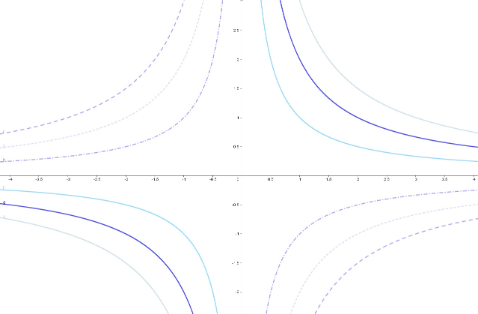
\includegraphics[width=0.5\textwidth]{fliadehiperbolas.png}
    \caption{Familia de hipérbolas}
\end{figure}

Dado un haz de curvas definidas por $\Phi(x,y,C)=0$, se puede obtener su ecuación diferencial asociada $F(x,y,y')=0$.
\\[5mm]
Las \textbf{trayectorias ortogonales} son aquellas curvas que cortan perpendicularmente a este haz original; su ecuación diferencial se obtiene simplemente reemplazando $y'$ por $-\frac{1}{y'}$ en la ED original, resultando en $F(x,y,-\frac{1}{y'})=0$.

\begin{figure}[H]
    \centering
        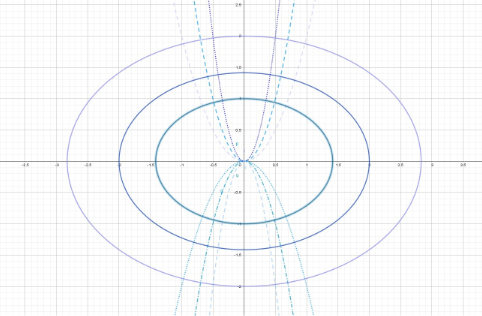
\includegraphics[width=0.5\textwidth]{trayortogonales.png}
    \caption{Trayectorias ortogonales a la familia de elipses concéntricas}
\end{figure}

\section{Envolvente de una familia de curvas}
La \textbf{envolvente} de una familia de curvas (parametrizada por $C$) es una curva en el plano $xy$ que es tangente a cada miembro de la familia en algún punto.
\\ [5mm]
Sea la familia de curvas definida por $\Phi(x,y,C)=0$. La envolvente se obtiene resolviendo el sistema:
\[
\begin{cases}
\Phi(x,y,C)=0 \\
\frac{\partial \Phi}{\partial C}=0
\end{cases}
\]

\begin{figure}[H]
    \centering
        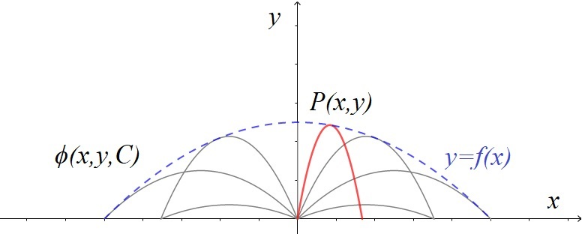
\includegraphics[width=0.5\textwidth]{curvaenvolvente.png}
    \caption{Representación gráfica de la curva envolvente (en rojo) de una familia de curvas (en azul)}
\end{figure}

\vspace{3mm}
\textbf{Relación con la Solución Singular:}
En las ED, la envolvente geométricamente representa a la \textbf{solución singular}. \\[5mm]
Al ser tangente en cada punto a una curva de la solución general, la envolvente comparte el mismo valor de la derivada ($y'$), por lo que satisface la ED original.
Sin embargo, se la llama "singular" porque es imposible obtenerla dándole un valor particular a $C$ de la solución general.

\section{Métodos de Resolución (ED de 1er Orden)}

\subsection{Variables Separables}
Son aquellas que tienen la forma $\frac{dy}{dx} = g(x)h(y) = \frac{g(x)}{h(y)} = \frac{h(y)}{g(x)}$.
Se resuelven agrupando cada variable con su respectivo diferencial e integrando directamente a ambos lados: $\int \frac{dy}{h(y)} = \int g(x)dx + C$.

\subsection{Ecuaciones Homogéneas}
Sea $f(x,y)$, es homogénea si al reemplazar $x$ y $y$ por $kx$ y $ky$ respectivamente, se obtiene
$$f(kx,ky) = k^n f(x,y) \forall k$$
Se resuelven aplicando la sustitución $v = \frac{y}{x}$ (lo que implica que $y = v \cdot x$), transformando la ecuación original en una nueva ED que sí es de variables separables.

\subsection{Lineales de Primer Orden}
Su forma estándar es $\frac{dy}{dx} + P(x)y = Q(x)$, siendo $P(x)$ y $Q(x)$ funciones exclusivas de $x$ o constantes.
\begin{itemize}
    \item Si $Q(x) = 0$, la ED es homogénea y se puede resolver separando variables.
    \item Si $Q(x) \neq 0$, se resuelve proponiendo una solución como el producto de dos funciones $y = u(x) \cdot v(x)$, resolviendo:
        $$ v(x) = e^{-\int P(x)dx} \qquad u = \int \frac{Q}{v} dx + C $$
\end{itemize}

\subsection{Ecuación de Bernoulli}
Son ED reducibles a lineales y tienen la forma $\frac{dy}{dx} + P(x)y = Q(x)y^n$, con $n \neq 0$ y $n \neq 1$.
Dividiendo toda la ecuación por $y^n$ se obtiene:
$$ y^{-n} \frac{dy}{dx} + P(x)y^{1-n} = Q(x) $$
Y se transforman en una ED Lineal clásica mediante la sustitución $t = y^{1-n}$:
$$ \frac{dt}{dx} + (1-n)P(x)t = (1-n)Q(x) $$

\subsection{Ecuaciones Exactas}
Es una ED de primer orden y primer grado. Parten de la diferencial total de una función y tienen la forma:
$$M(x,y)dx + N(x,y)dy = 0$$
Si ambas son continuas, derivables y se cumple la igualdad de sus derivadas parciales cruzadas: $\frac{\partial M}{\partial y} = \frac{\partial N}{\partial x}$, es una \textbf{ED exacta} y la solución general es:
$$u(x,y) = C$$

\subsection{Reducción a ED Exactas (Factor Integrante)}
Si una ED de la forma $M(x,y)dx + N(x,y)dy = 0$ \textbf{no es exacta} ($\frac{\partial M}{\partial y} \neq \frac{\partial N}{\partial x}$), a menudo es posible convertirla en una ecuación exacta multiplicándola por el \textbf{factor integrante} ($\mu$).
\\[3mm]
Para hallar este factor, se presentan dos casos principales:
\begin{itemize}
    \item \textbf{Factor dependiente solo de $x$:} Si la expresión $\frac{\frac{\partial M}{\partial y} - \frac{\partial N}{\partial x}}{N}$ depende únicamente de la variable $x$ (o es una constante), entonces el factor integrante se calcula como:
    $$ \mu(x) = e^{\int \frac{\frac{\partial M}{\partial y} - \frac{\partial N}{\partial x}}{N} dx} $$

    \item \textbf{Factor dependiente solo de $y$:} Si la expresión $\frac{\frac{\partial N}{\partial x} - \frac{\partial M}{\partial y}}{M}$ depende únicamente de la variable $y$ (o es una constante), el factor integrante será:
    $$ \mu(y) = e^{\int \frac{\frac{\partial N}{\partial x} - \frac{\partial M}{\partial y}}{M} dy} $$
\end{itemize}

Una vez calculado $\mu$, se multiplica toda la ecuación diferencial original por este factor. La nueva ecuación resultante $\mu M dx + \mu N dy = 0$ será exacta y se resolverá con el método tradicional.

Observaciones:
\begin{itemize}
    \item Si la ED es homogénea y $Mx + Ny \neq 0 \Rightarrow \frac{1}{Mx + Ny}$ es un \textbf{factor integrante} de la ED.
    \item Si la ED es de la forma $yP(x,y)dx + xQ(x,y)dy = 0$ y $P(x,y) \neq Q(x,y) \Rightarrow \frac{1}{xy[P(x,y)-Q(x,y)]} = \frac{1}{Mx + Ny}$ es un \textbf{factor integrante} de la ED.
\end{itemize}

\newpage
\part{Ecuaciones Diferenciales Lineales de Orden Superior}

\section{Ecuaciones Diferenciales Lineales Homogéneas}
Una ecuación diferencial lineal de primer grado es \textbf{homogénea} si se puede escribir de la forma:
$$ a_0(x)y^{(n)} + a_1(x)y^{(n-1)} + \dots + a_n(x)y = 0 $$
Donde $a_i(x)$ son coeficientes dependientes de la variable independiente $x$ y $a_0(x) \neq 0$.
\\El término independiente (a la derecha) es estrictamente cero.

\textbf{Teorema (Principio de Superposición):}
Si $y_1, y_2, \dots, y_k$ son soluciones de una ecuación diferencial lineal homogénea en un intervalo $I$, entonces cualquier combinación lineal de estas funciones también es una solución en $I$. Es decir:
$$ y = c_1y_1 + c_2y_2 + \dots + c_ky_k $$
donde $c_1, c_2, \dots, c_k$ son constantes arbitrarias.
\\[5mm]
Dos soluciones $y_1$ y $y_2$ de una ecuación diferencial lineal homogénea son \textbf{linealmente independientes} si no existe un número constante $k$ tal que $y_1 = ky_2$. En caso contrario, se dice que son \textbf{linealmente dependientes}.

\subsubsection{Wronskiano}
El \textbf{Wronskiano} es una herramienta utilizada para determinar la independencia lineal de un conjunto de funciones. Para dos funciones $y_1$ y $y_2$, el Wronskiano se define como:
$$ W(y_1, y_2) = \begin{vmatrix}
y_1 & y_2 \\
y_1' & y_2'
\end{vmatrix} $$
Si $W(y_1, y_2) \neq 0$ en algún punto del intervalo considerado, entonces $y_1$ y $y_2$ son \textbf{linealmente independientes}. Si el Wronskiano es cero en todo el intervalo, entonces las funciones son \textbf{linealmente dependientes}.

%Caja de texto: Teorea de Liouville
\begin{tcolorbox}[colback=blue!5!white,colframe=blue!75!black,title=Teorema de Liouville]
$$ W(x) = Ce^{-\int_{x_0}^{x} a_{1}dx} = w_0e^{-\int_{x_0}^{x} a_{1}dx}$$
\end{tcolorbox}


\section{Ecuaciones Diferenciales Lineales Homogéneas de Segundo Orden}
La forma general con coeficientes constantes es:
$$ ay'' + by' + cy = 0 $$
Para resolverla, se asume una solución de la forma $y = e^{rx}$, lo que lleva a la \textbf{ecuación característica} o ecuación auxiliar:
$$ ar^2 + br + c = 0 $$
Las raíces de este polinomio de segundo grado determinan la forma de la solución general. Existen tres casos posibles dependiendo del discriminante $\Delta = b^2 - 4ac$:

\begin{itemize}
    \item \textbf{Caso 1: Raíces reales y distintas ($\Delta > 0$).}
    Si $r_1$ y $r_2$ son raíces reales tales que $r_1 \neq r_2$, la solución general es:
    $$ y(x) = c_1e^{r_1x} + c_2e^{r_2x} $$

    \item \textbf{Caso 2: Raíces reales y repetidas ($\Delta = 0$).}
    Si $r_1 = r_2 = r$, la solución general incluye un factor multiplicativo $x$ para asegurar la independencia lineal:
    $$ y(x) = c_1e^{rx} + c_2xe^{rx} $$

    \item \textbf{Caso 3: Raíces complejas conjugadas ($\Delta < 0$).}
    Si las raíces son de la forma $r = \alpha \pm \beta i$, la solución general (utilizando la fórmula de Euler) es:
    $$ y(x) = e^{\alpha x} (c_1 \cos(\beta x) + c_2 \sin(\beta x)) $$
\end{itemize}

\section{Ecuaciones Diferenciales Lineales Homogéneas de Enésimo Orden}
Se generalizan los conceptos aplicados en las de segundo orden. Para una ED de la forma:
$$ y^{(n)} + a_{1} y^{(n-1)} + \dots + a_{n-1} y = 0 $$
Se plantea la ecuación característica de grado $n$:
$$ r^n + a_{1} r^{n-1} + \dots + a_{n-1} r = 0 $$
La solución general es una combinación lineal de $n$ soluciones linealmente independientes.
\begin{itemize}
    \item \textbf{Raíces reales distintas:}
            $$ y = C_1e^{r_1x} + C_2e^{r_2x} + \dots + C_ne^{r_nx} $$
    \item \textbf{Raíces reales repetidas:}
            $$ y = C_1e^{rx} + C_2xe^{rx} + \dots + C_m x^{m-1}e^{rx} $$
    \item \textbf{Raíces complejas conjugadas:}
            $$ y = e^{\alpha x} (C_1 \cos(\beta x) + C_2 \sin(\beta x)) + \dots + e^{\alpha x} (C_{2m-1} \cos(\beta x) + C_{2m} \sin(\beta x)) $$
\end{itemize}

\textbf{Definición (Wronskiano):}
Un conjunto de funciones $\{y_1, y_2, \dots, y_n\}$ es \textbf{linealmente independiente} en un intervalo $I$ si y solo si su Wronskiano no es nulo ($W \neq 0$) en $I$.
$$ W(y_1, y_2, \dots, y_n) = \begin{vmatrix}
y_1 & y_2 & \dots & y_n \\
y_1' & y_2' & \dots & y_n' \\
\vdots & \vdots & \ddots & \vdots \\
y_1^{(n-1)} & y_2^{(n-1)} & \dots & y_n^{(n-1)}
\end{vmatrix} $$

\section{Ecuaciones Diferenciales Lineales No Homogéneas}
Tienen la forma:
$$ y'' + py' + qy = f(x)$$
Donde $f(x) \neq 0$ y $p$, $q$ son constantes.
\\[5mm]
\textbf{Teorema de la Solución General:}
La solución general $y(x)$ de una ecuación lineal no homogénea es la suma de la \textbf{solución homogénea} $y_h(x)$ y una \textbf{solución particular} $y_p(x)$ cualquiera de la ecuación no homogénea completa.
$$ y(x) = y_h(x) + y_p(x) $$

\section{Método de los Coeficientes Indeterminados}
Es una técnica heurística para hallar una solución particular $y_p(x)$ de una ecuación diferencial lineal no homogénea con coeficientes constantes.
\\[5mm]
\textbf{Condiciones de aplicabilidad:}
El método solo funciona si $f(x)$ es una función de tipos específicos:
\begin{itemize}
    \item Polinomios (ej., $x^2 + 3$).
    \item Funciones exponenciales (ej., $e^{3x}$).
    \item Senos y cosenos (ej., $\sin(2x), \cos(4x)$).
    \item Sumas y productos finitos de las anteriores.
\end{itemize}

\textbf{Reglas del Método:}
\begin{enumerate}
    \item \textbf{Regla Básica:} Si $f(x)$ pertenece a uno de los tipos permitidos, se asume una solución particular $y_p$ que sea una combinación lineal de los términos de $f(x)$ y de todas sus derivadas linealmente independientes.
    \begin{itemize}
        \item Si $f(x) = P_n(x)$, se asume $y_p = A_nx^n + \dots + A_1x + A_0$.
        \item Si $f(x) = e^{kx}$, se asume $y_p = A e^{kx}$.
        \item Si $f(x) = \sin(kx)$ o $\cos(kx)$, se asume $y_p = A\cos(kx) + B\sin(kx)$.
    \end{itemize}
    \item \textbf{Regla de Modificación (Multiplicación):} Si algún término de la forma propuesta para $y_p$ resulta ser solución de la ecuación \textbf{homogénea asociada} (es decir, forma parte de $y_h$), entonces la forma propuesta para $y_p$ debe multiplicarse por $x^s$, donde $s$ es el menor entero positivo que elimine la duplicación con cualquier término de $y_h$.
\end{enumerate}
Una vez establecida la forma general de $y_p$, se deriva las veces necesarias, se sustituye en la ED original y se igualan los coeficientes de funciones semejantes en ambos lados de la igualdad para determinar el valor exacto de las constantes ("coeficientes indeterminados").

\subsection{Tabla del método de los coeficientes indeterminados}
\begin{figure}[H]
    \centering
        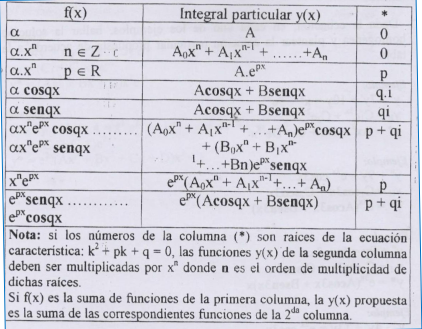
\includegraphics[width=0.5\textwidth]{coefindet.png}
    \end{figure}


 % --- Continuación del documento ---

 \section{Método de Variación de Parámetros}
 Es un método más general que el de coeficientes indeterminados, ya que permite hallar $y_p$ para cualquier función $f(x)$ continua, no solo polinomios o exponenciales.
 \\[3mm]
 Para una ED de segundo orden $y'' + p(x)y' + q(x)y = f(x)$, si $y_h = C_1y_1 + C_2y_2$, proponemos:
 $$ y_p = u_1(x)y_1 + u_2(x)y_2 $$
 Donde las funciones $u_1$ y $u_2$ se determinan resolviendo el sistema:
 \[
 \begin{cases}
 u_1'y_1 + u_2'y_2 = 0 \\
 u_1'y_1' + u_2'y_2' = f(x)
 \end{cases}
 \]
 Utilizando la regla de Cramer y el Wronskiano ($W$):
 $$ u_1' = \frac{-y_2 f(x)}{W(y_1, y_2)} \quad ; \quad u_2' = \frac{y_1 f(x)}{W(y_1, y_2)} $$
 Finalmente, se integran $u_1'$ y $u_2'$ para obtener $y_p$.

 \section{Sistemas de Ecuaciones Diferenciales Lineales}
 Un sistema de $n$ ecuaciones diferenciales de primer orden tiene la forma:
 \[
 \begin{cases}
 \frac{dx_1}{dt} = a_{11}x_1 + a_{12}x_2 + \dots + a_{1n}x_n + f_1(t) \\
 \vdots \\
 \frac{dx_n}{dt} = a_{n1}x_1 + a_{n2}x_2 + \dots + a_{nn}x_n + f_n(t)
 \end{cases}
 \]
 Si todas las $f_i(t) = 0$, el sistema es \textbf{homogéneo}.

 \subsection{Método de los Operadores (Eliminación)}
 Consiste en utilizar el operador diferencial $D = \frac{d}{dt}$ para escribir el sistema como un sistema de ecuaciones algebraicas y eliminar variables hasta obtener una sola ED de orden superior en una sola variable.

 \subsection{Sistemas Homogéneos con Coeficientes Constantes}
 Buscamos soluciones de la forma $\mathbf{X} = \mathbf{V}e^{\lambda t}$, donde $\mathbf{V}$ es un vector de constantes. Esto conduce a un problema de \textbf{autovalores y autovectores}:
 $$ (A - \lambda I)\mathbf{V} = 0 $$
 Donde $A$ es la matriz de coeficientes. La naturaleza de los autovalores $\lambda$ determina la solución:
 \begin{itemize}
     \item \textbf{Autovalores reales y distintos:} $\mathbf{X} = C_1 \mathbf{V_1} e^{\lambda_1 t} + \dots + C_n \mathbf{V_n} e^{\lambda_n t}$.
     \item \textbf{Autovalores complejos:} Si $\lambda = \alpha \pm \beta i$, la solución involucra senos y cosenos multiplicados por $e^{\alpha t}$.
 \end{itemize}

 \section{Reducción de una ED de orden $n$ a un sistema}
 Cualquier ecuación diferencial de orden $n$:
 $$ y^{(n)} = F(t, y, y', \dots, y^{(n-1)}) $$
 Puede transformarse en un sistema de $n$ ecuaciones de primer orden mediante el siguiente cambio de variables:
 \begin{multicols}{2}
 \begin{itemize}
     \item $x_1 = y$
     \item $x_2 = y'$
     \item $x_3 = y''$
     \item $\dots$
     \item $x_n = y^{(n-1)}$
 \end{itemize}
 \columnbreak
 \textbf{Resultando en:}
 \begin{itemize}
     \item $x_1' = x_2$
     \item $x_2' = x_3$
     \item $\dots$
     \item $x_n' = F(t, x_1, x_2, \dots, x_n)$
 \end{itemize}
 \end{multicols}

 \newpage
 \part{Transformada de Laplace}

 \section{Definición y Propiedades}
 Sea $f(t)$ una función definida para $t \geqslant 0$, la transformada de Laplace se define como:
 \begin{tcolorbox}[colback=red!5!white,colframe=red!75!black,title=Definición Integral]
 $$ \mathcal{L}\{f(t)\} = F(s) = \int_{0}^{\infty} e^{-st} f(t) dt $$
 \end{tcolorbox}

 \subsection{Condiciones de Existencia}
 Para que $\mathcal{L}\{f(t)\}$ exista, $f(t)$ debe ser:
 \begin{enumerate}
     \item \textbf{Continua por tramos} en el intervalo $[0, \infty)$.
     \item \textbf{De orden exponencial:} Existen constantes $M > 0, c$ y $T > 0$ tales que $|f(t)| \le Me^{ct}$ para todo $t > T$.
 \end{enumerate}

 \subsection{Propiedades Principales}
 \begin{itemize}
     \item \textbf{Linealidad:} $\mathcal{L}\{af(t) + bg(t)\} = aF(s) + bG(s)$.
     \item \textbf{Primer Teorema de Traslación:} $\mathcal{L}\{e^{at}f(t)\} = F(s-a)$.
     \item \textbf{Transformada de la Derivada:}
     $$ \mathcal{L}\{f'(t)\} = sF(s) - f(0) $$
     $$ \mathcal{L}\{f''(t)\} = s^2F(s) - sf(0) - f'(0) $$
     Esta propiedad es la que permite resolver ED transformándolas en ecuaciones algebraicas.
 \end{itemize}

 \newpage
 \section{Transformada Inversa y Fracciones Simples}
 Para recuperar $f(t)$ a partir de $F(s)$, se utiliza la transformada inversa $\mathcal{L}^{-1}\{F(s)\}$. El método más común es la descomposición en \textbf{fracciones simples} para llevar la expresión a formas tabuladas.

 \begin{table}[h]
 \centering
 \begin{tabular}{@{}lll@{}}
 \toprule
 $f(t)$ & $F(s)$ & Restricciones \\ \midrule
 $1$ & $1/s$ & $s > 0$ \\
 $t^n$ & $n!/s^{n+1}$ & $n=1,2 \dots$ \\
 $e^{at}$ & $1/(s-a)$ & $s > a$ \\
 $\sin(kt)$ & $k/(s^2+k^2)$ & $s > 0$ \\
 $\cos(kt)$ & $s/(s^2+k^2)$ & $s > 0$ \\ \bottomrule
 \end{tabular}
 \caption{Transformadas básicas frecuentes}
 \end{table}

 \end{document}
